\chapter					{Über \TeX}														\renewcommand*{\authorOfNextLines}{Helmut Quinz}
\TeX ~ist ein von Donald E. Knuth ab 1977 entwickeltes und 1986 fertiggestelltes Textsatzsystem.
Hauptfunktion ist das grafisch ansprechende komponieren von Text und Grafiken.
Das \TeX -Grundpaket verfügt über eine Makrosprache um den Text-Satz beeinflussen zu können.
Die Entwicklung des \TeX -Grundpaketes gilt, abgesehen von der Behebung unerwünschten Verhaltens als abgeschlossen.
\TeX wird nicht zuletzt auf Grund der guten Unterstützung bei der Darstellung mathematischer Zusammenhänge im technisch-universitären Bereich verwendet.
Das Textsatzsystem wird von einer akttiven Gemeinschaft getragen die für dieses System eine Unzahl an Makrosammlungen bereitstellen und weiterentwickeln.
Diese Makrosamlungen sind wie das \TeX -Grundpaket frei verfügbar. 
Heute wird \TeX ~üblicherweise eingebunden in leistungsfähige Erweiterungspakete verwendet. 
Bekanntestes, wenn auch nicht alleinstehendes Beispiel dafür ist \LaTeX.
\TeX ~ist rechnerunabhängig verwendbar und sollte auf allen Betriebssystemen vergleichbare Ergebnisse liefern.\\

\TeX ~wird heute von verschiedenen Distributoren zur Verfügung gestellt.
Dazu gehören
\begin{itemize}
	\item MiKTeX,
	\item TeX Live oder
	\item teTex (wird seit Mai 2006 nicht mehr weiterentwickelt) 
\end{itemize}

Die Pakete stellen jeweils unterschiedliche Compiler-Sätze bereit, welche sich aus der historischen Entwicklung des Textsatzsystems erklären lassen.
so wurde LaTeX, welches in der Grundeinstellung \texttt{.DVI} Dateien erstellt zu PdfLaTeX weiterentwickelt.
Letzteres wurde unter Berücksichtigung aktueller Entwicklungen (utf8 als Standart-Zeichensatz) zu LuaLaTex und XeLatTex erweitert.
	\section				{Über \TeX -Dokumente}
		\subsection 		{Formatierung von \TeX -Dateien}								\renewcommand*{\authorOfNextLines}{Helmut Quinz}
Der \gqq{Quellcode} für \TeX oder \LaTeX Dokumente sind einfache Textdateien, erweitert durch Formatierungsangaben.
Die Zeichenkodierung dieser Textdateien muss dem Satzsystem bekannt sein.
Aktuelle Pakete verwenden \texttt{UTF8} als Standard.
Die Verwendung dieser Zeichenkodierung wird empfohlen.\\

Grundsätzlich können \TeX -Dateien mit jedem Text- oder Code-Editor erstellt werden.
Das Übersetzen der Dokumente ist auch mit Konsolen-Befehlen möglich (\seeRefNamePage{par:UebersetzenKonsole}).
Die Verwendung von eigenen \TeX -Editoren beziehungsweise Code-Editoren mit \TeX Unterstützung scheint aber empfehlenswert. 
Diese bieten meist einfach zu bedienende Assistenten sowie die Möglichkeit mit eigenen Text-Makros zu arbeiten an.
Darüber hinaus stellen diese meist eine schnelle Navigation zwischen den Textdateien und dem PDF-Dokument bereit.
		\subsection 		{Dokumentklassen}												\renewcommand*{\authorOfNextLines}{Helmut Quinz}
Für \TeX -(Haupt)dokumente ist eine Dokumentklasse zu definieren.
Diese Definition steht am Beginn jedes Hauptdokuments!.
Die Dokumentklasse entscheidet unter anderem welche Makros insbesondere bezüglich der Dokumentstrukturierung zu Verfügung stehen.
Neben den von \TeX definierten Dokumentklassen lassen sich zusätzliche über Makropakete bereitgestellte Klassen mit speziellen Eigenschaften verwenden.
Besonders erwähnenswert ist dabei KOMA-Skript. 
\TeX und seine Erweiterungen sind auf den Bedarf des US-Amerikanischen Raums zugeschnitten. 
Der Entwickler Markus Kohm hat \LaTeX ~mit seinem Makro-Paket auf europäische, insbesondere deutschsprachige Verhältnisse angepasst.
Sein Paket wird aber mittlerweile aufgrund seiner Flexibilität auch gerne außerhalb Europas verwendet.\\

Für den Schulgebrauch wichtige Dokumentklassen sind: 
\begin {table} [ht]
\stretchTableRows{1.2}
\begin{tabular}{p{20mm}p{25mm}p{100mm}}
	\TeX Klasse & KOMA-Klasse 	& Anwendung\\
	article 	& scrartcl		& kleine Dokumente wie Hausaufgaben oder Protokolle\\ 
	report		& scrreprt		& Umfangreiche Dokumente wie Abschlussarbeiten oder Skripta\\
	book		& scrbook		& SEHR umfangreiche Dokumente die Buch-Stärke erreichen\\
	letter		& scrlttr2		& Briefe\\
	slides		&				& Präsentationen\\
	
\end{tabular}
\caption {Wichtige \LaTeX -Dokumentklassen}
\end {table}
\FloatBarrier
Am auffälligsten unterscheiden sich die Klassen \emph{article} \emph{report} und \emph{book} durch die Bereitstellung von Strukturierungsangaben.
Diese Strukturierungsangaben legen Dokumenthierarchien insbesondere für die Inhaltsangabe fest.
Folgende Gliederungsmerkmale stehen zur Verfügung
\begin {table} [ht]
\stretchTableRows{1.2}
\begin{tabular}{clccc}
	Level	& Ebene 					& \multicolumn{3}{c}{Verfügbar in }\\
			&							& (scr)article 	& (scr)report 	& (scr)book	\\
	-1		& \verb|\part| 				& ---			& ---			& X\\ 
	0		& \verb|\chapter|			& ---			& X				& X\\ 
	1		& \verb|\section| 			& X				& X				& X\\ 
	2		& \verb|\subsection| 		& X				& X				& X\\ 
	3		& \verb|\subsubsection| 	& X				& X				& X\\ 
	4		& \verb|\paragraph|		 	& X				& X				& X\\ 
	5		& \verb|\subparagraph|	 	& X				& X				& X\\ 
	
\end{tabular}
\caption {Gliederungsebenen in \LaTeX}
\end {table}
\FloatBarrier
	\section				{Übersetzen eines \TeX -Dateien mit Konsolen-Befehlen}			\renewcommand*{\authorOfNextLines}{Helmut Quinz}
\label{par:UebersetzenKonsole}
Das Übersetzen des Dokuments aus der Konsole ist mit dem Befehl\\
\begin{center} \texttt{lualatex} \emph{Dateiname}\\ \end{center}
möglich.
	\section				{Über diese Vorlage}
	\section				{Verwendete Systeme}											Diese Vorlage ist unter Verwendung der Distribution \href{https://www.tug.org/texlive/}{TeX Live} mit dem Compiler LuaLaTex erstellt worden.\\
Als Editor hat sich der Autor dieser Zeilen an \href{https://www.texstudio.org/}{TeXstudio} gewöhnt. 
Er wird als Open-Source-Projekt entwickelt und steht sowohl für Windows als auch für Linux zur Verfügung.
Die (wenigen) Editor-Beschreibungen dieses Dokuments beziehen sich auf TeXstudio.
Es ist aber sehr wahrscheinlich, dass beschriebene Einstellungen und Funktionen auch in anderen \TeX -Editoren zu finden sind.\\

Die Schriftart \gqq{ARIAL} ist unter Windows grundsätzlich verfügbar. 
Unter Linux muss sie installiert werden.
		\subsection 		{Installieren von Microsoft-Schriftarten ARIAL unter Linux}		\renewcommand*{\authorOfNextLines}{Helmut Quinz}
Um Microsoft\textcopyright ~Fonts wie \emph{ARIAL} unter Linux verfügbar zu stellen ist in einer Konsole wie folgt zu installieren:\\
\texttt{sudo apt install ttf-mscorefonts-installer}\\
\texttt{sudo fc-cache -f}\\

Eine Überprüfung der Implementierung ist mittels\\
\texttt{fc-match Arial}\\
möglich.
	\section				{Erforderliche Einstellungen für \TeX ~Editoren}				\renewcommand*{\authorOfNextLines}{Helmut Quinz}
Wesentlich für das Generieren des PDF-Dokumentes sind die Einstellungen für den Standardcompiler sowie das Standard-Bibliographieprogramm.
Als Compiler ist \gqq{\texttt{LuaLaTeX}} zu verwenden, für die Bibliographie \gqq{\texttt{Biber}}
\begin{figure}[ht]
	\begin{overpic}[width=130mm,abs,unit=1mm,,tics=10]{../13_D3/VorlageEinstellungenUebersetzen.png}
		\put(26,2)		{\opFrame				[white, rounded corners=1mm]{35mm,3mm}}
		\put(26,11.5)		{\opFrame				[white, rounded corners=1mm]{35mm,3mm}}
	\end{overpic}	
	\caption{\TeX -Editor Einstellungen für das Übersetzen}
\end{figure}
\FloatBarrier
Die Zeichenkodierung der Text-Dateien sollte in Grundeinstellung auf \texttt{utf8} gestellt sein. 
Es schadet jedoch nicht dies zu kontrollieren:
\begin{figure}[ht]
	\begin{overpic}[width=130mm,abs,unit=1mm,,tics=10]{../13_D3/VorlageEinstellungenEditor.png}
		\put(36,10)		{\opFrame				[white, rounded corners=1mm]{50mm,3mm}}
	\end{overpic}	
	\caption{\TeX -Editor Einstellungen für das Erstellen der Dateien}
\end{figure}
\FloatBarrier
	\section				{Die Struktur dieser Vorlage}									\renewcommand*{\authorOfNextLines}{Helmut Quinz}
Der Speicherort der zu dieser Vorlage gehörenden Dateien ist unerheblich.
Es empfiehlt sich aber ein Verzeichnis auf einem Cloud-Speicher zu verwenden.
Das reduziert die Gefahr Daten zu verlieren und ermöglicht dezentrales Arbeiten.
Innerhalb des Verzeichnisses wird empfohlen folgende Struktur beizubehalten:
\begin{figure} [ht]
	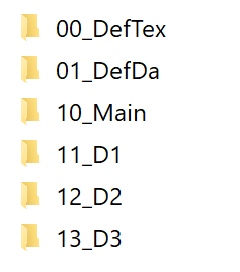
\includegraphics{../13_D3/VorlageDateistruktur.png} 
	\caption{Verzeichnisstruktur dieser Vorlage}
\end{figure}
\FloatBarrier
Die Verzeichnisse sind wie folgt festgelegt:
\begin {table} [ht]
\stretchTableRows{1.3}
\begin{tabular}{p{20mm}p{37mm}p{90mm}}
	Verzeichnis 		& Inhalt  	& Bemerkung\\ \hline
	\texttt{00\_DefTex}	& Für den Aufbau des Dokuments relevante Definitionen 
		& Der Verzeichnisname wird von der Vorlage referenziert und darf nicht verändert werden.
		  Der Inhalt des Ordners ist nur in Ausnahmefällen zu ändern.\\
	\texttt{01\_DefDa}	& Einstellungen zur \typeOfWork ~.  
		& Der Verzeichnisname wird von der Vorlage referenziert und darf nicht verändert werden.
		  Der Inhalt der Dateien in diesem Ordner ist vom Anwender der Arbeit entsprechend anzupassen.\\
	\texttt{10\_Main}	& Hauptdokument	
		& Änderungen im Verzeichnis- und Dokumentnamen haben bei korrektem Arbeiten keine Auswirkung.
		  Das Hauptdokument muss jedoch direkt in einem Unterverzeichnis abgelegt sein.\\
	\texttt{11\_D1}	& von den Anwendern erstellte Dateien, Inhalt der \typeOfWork .	
		& Änderungen im Verzeichnis- und Dokumentnamen haben bei korrektem Arbeiten keine Auswirkung.
		  Die Strukturierung ist nur ein Vorschlag des Autors. 
		  Die einzelnen Dokumente können auch unter \texttt{10\_Main} abgelegt sein.\\
\end{tabular}
\caption {Inhalt der Verzeichnisse dieser Vorlage}
\end {table}
\FloatBarrier
Grundsätzlich ist das Schreiben der kompletten \typeOfWork ~im Hauptdokument möglich.
Es erscheint jedoch praktikabel mehrere kleine Dateien zum Einbinden in das Hauptdokument anzulegen. 
Dies gestaltet Anpassungen der in Dokumentstruktur während dem Erstellen der Dokumentation einfacher!

\subsubsection{Hinweis:}
Anders als bei Windows-Systemen ist unter Linux die korrekte Groß- und Kleinschreibung bei Verzeichnis- und Dateinamen für das Finden der Dateien durch den Compiler relevant!
		\subsection			{Die Dateien in \texttt{00\_DefTex}}							\renewcommand*{\authorOfNextLines}{Helmut Quinz}
\begin {longtable} [ht] {p{40mm}p{110mm}}
\stretchTableRows{1.3}
	Datei 				 		& Inhalt\\ \hline
	\endhead
	\hline
	\endfoot
	\endlastfoot

	\texttt{0Präambel}			& Bindet die weiteren zur Gestaltung des Dokuments erforderlichen Dateien ein.\\
	\texttt{CompilerOptions}	& Legt Vorgaben für das Generieren des Dokuemnts fest\\
	\texttt{DefColors}			& Definition einiger nicht in eingebundenen Paketen enthaltener Farben. 
								  Eine Anpassung durch den Anwender ist unproblematisch.\\
	\texttt{DefMakrosAllgemein}	& Definition im Dokument verwendeter selbst erstellter Makros.
								  Eine Anpassung sollte nur von erfahrenen Anwendern vorgenommen werden.\\
	\texttt{DefPackages}		& Einbindung von Makro-Paketen.
								  Eine Anpassung sollte nur von erfahrenen Anwendern vorgenommen werden.\\
	\texttt{DefStyleDA}			& Festlegung der optischen Gestaltung.
								  Eine Anpassung sollte nur von erfahrenen Anwendern vorgenommen werden.\\
	\texttt{DoAbstract}			& Erstellen der Kurzbeschreibung.
								  Eine Anpassung sollte nur von erfahrenen Anwendern vorgenommen werden.\\
	\texttt{DoAbstractEnglish}	& Aufbau der Kurzbeschreibung in Englisch
								  Eine Anpassung sollte nur von erfahrenen Anwendern vorgenommen werden.\\
	\texttt{DoAbstractGerman}	& Aufbau der Kurzbeschreibung in Deutsch
								  Eine Anpassung sollte nur von erfahrenen Anwendern vorgenommen werden.\\
	\texttt{DoTitle}			& Erstellen der Titelseite
								  Eine Anpassung sollte nur von erfahrenen Anwendern vorgenommen werden.\\
	\texttt{TitleHelpers}		& Makros die beim Erstellen der Titelseite unterstützen.
								  Eine Anpassung sollte nicht erforderlich sein.\\
\caption {Dateien im Verzeichnis \texttt{00\_DefTex}}
\end {longtable}
\FloatBarrier
\subsubsection{Hinweis:}
Die Bilddateien in diesem Ordner werden beim Übersetzen des Dokuments eingebunden.
\newpage
		\subsection			{Die Dateien in \texttt{01\_DefDa}}								\renewcommand*{\authorOfNextLines}{Helmut Quinz}
\begin {longtable} [ht] {p{40mm}p{110mm}}
\stretchTableRows{1.3}
	Datei				 		& Inhalt\\ \hline
	\endhead
	\hline
	\endfoot
	\endlastfoot

	\texttt{Acronyme}			& Kleine Makros um beim Schreiben des Textes mit Abkürzungen arbeiten zu können.
								  Die Anpassung durch den Anwender nach bestehenden Muster ist möglich\\
	\texttt{Anhang}				& Aufbau des Dokument-Anhangs.
								  Eine Anpassung sollte nicht erforderlich sein.\\
	
	\texttt{DefKurzfassung}		& Festlegung der Texte und Bilder für die Kurzfassung. 
								  Eine Anpassung durch den Anwender ist zwingend erforderlich.\\
	\texttt{DefNamenUndDaten}	& Festlegung von Eckdaten der \typeOfWork
								  Eine Anpassung durch den Anwender ist zwingend erforderlich.\\
	\texttt{Quellenverweise}	& Definition verwendeter Quellen.
								  Eine Anpassung durch den Anwender ist zwingend erforderlich.
								  Bitte Erarbeite Sie sich die Regel zur Definition der Bibliographie selbst.\\
	\texttt{Vorwort}			& Vorwort der \typeOfWork.
								  Eine Anpassung durch den Anwender ist zwingend erforderlich.\\
\caption {Dateien im Verzeichnis \texttt{01\_DefDa}}
\end {longtable}
\FloatBarrier
			\subsubsection	{Hinweis zum Makro \texttt{\textbackslash department}}			\renewcommand*{\authorOfNextLines}{Helmut Quinz}
Die Vorlage verwendet das Makro \textbackslash  department zum Erstellen der ersten Kopfzeile sowie der Art der Arbeit (Abschlussarbeit, Diplomarbeit).
Das Makro soll aufgelöst eine Festpunktzahl zurückgeben wobei die Werte wie folgt interpretiert werden:
\begin {table} [ht]
\stretchTableRows{1.2}
\begin{tabular}{cll}
	0	& Fachschule Mechatronik\\
	1	& Höhere Abteilung für Wirtschaftsingenieurwesen\\
	2	& Höhere Abteilung für Elektrotechnik Schwerpunkt Automatisierungstechnik\\
	3	& Höhere Abteilung für Elektrotechnik Schwerpunkt Informationstechnologie\\
	4	& Höhere Abteilung für Maschinenbau Schwerpunkt Umwelttechnik\\ 
	5	& Höhere Abteilung für Maschinenbau Schwerpunkt Anlagentechnik\\
	6	& Höhere Abteilung für Maschinenbau Schwerpunkt Automatisierungstechnik\\ 
	7	& Höhere Abteilung für Informationstechnologie\\
\end{tabular}
\caption {Zulässige Werte für das Makro \textbackslash  department}
\end {table}
\FloatBarrier
			\subsubsection	{Definition der Studierenden}									\renewcommand*{\authorOfNextLines}{Helmut Quinz}
in der Datei \texttt{DefNamenUndDaten.tex} sind unter anderem die, an der \typeOfWork beteiligten Personen anzugeben.
Dies gescheit über die Makros
\begin{itemize}
	\item \textbackslash studentNameI bis \textbackslash studentNameV
	\item \textbackslash studentGradeI bis \textbackslash studentGradeV
	\item \textbackslash supervisorNameI bis \textbackslash supervisorNameV
\end{itemize}

Für jedes dieser Makros ist zumindest jenes mit der römischen Nummerierung \texttt{I} zu definieren.
Ist für einen Studenten kein eigener Betreuer (subervisor) definiert wählt das System automatisch den \textbackslash supervisorNameI.
Nicht benötigte Definitionen können aus der Datei gelöscht werden.
		\subsection			{Haupt- und Subdokumente}										\renewcommand*{\authorOfNextLines}{Helmut Quinz}
Möchten Sie wie vom Autor empfohlen mit Unterdokumenten arbeiten sind diese mit dem Befehl\\
\verb|\input{Pfad/Dateiname.erweiterung}|\\
einzubinden.\\
Die Pfadangaben sind \textbf{relativ zum Hauptdokument} zu gestalten.
Das Verzeichnis des Hauptdokuments ist mit \verb|./| anzugeben.
Um in der Verzeichnisstruktur eine Hierarchie höher zu springen dient die Angabe \verb|../|.
Dies kann auch gestapelt werden so wechselt \verb|../../| um zwei Ebenen nach oben.
Die Strukturierung Ihres Inhaltes bleibt Ihnen überlassen. 
Die Empfehlung eher mit mehreren kleinen Dokumenten (50 bis 100 Zeilen) zu arbeiten bleibt aber aufrecht.
	\section				{Die Abfrage \texttt{\textbackslash ifCompileFinal}}			\renewcommand*{\authorOfNextLines}{Helmut Quinz}
Im Hauptdokument finden Sie die Definition\\
\verb|\newif\ifCompileFinal\CompileFinalfalse|\\
Damit wird festgelegt, ob das Dokument als noch zu bearbeitende Version übersetzt werden soll oder als final abzugebend.
In ersterem Fall zeigt der Compiler durch schwarze Rechtecke welchen Stellen der Text über die festgelegte Breite hinaus gesetzt wurde.
Hier ist in der Textkomposition manuell nachzuarbeiten.\\
Zusätzlich zeigt so das Dokument im Anhang die vom Paket \texttt{fixme} erkannten Anmerkungen an.\\

Die Umstellung zwischen den Versionen erfolgt über die Angabe 
\begin{description}
	\item[\texttt{\textbackslash CompileFinalfalse}] für eine noch zu bearbeitende Version \bzw
	\item[\texttt{\textbackslash CompileFinaltrue}] für die finale Version 
\end{description}
\subsubsection{Hinweis}
Findet der Compiler mit \verb|\fxfatal| definierte Anmerkungen lässt sich das Dokument nicht in seiner finalen Version erstellen!
	\section				{Das Makro \texttt{\textbackslash authorOfNextLines}}			\renewcommand*{\authorOfNextLines}{Helmut Quinz}
Die Vorlage trägt den Inhalt des Makros \verb|\authorOfNextLines| in der Fußzeile ein.
duch dieses Makro sollte der Ersteller eines Dokumenteils leichter identifizierbar sein.
Verändert wird der Inhalt des Makros mit dem Befehl \verb|\renewcommand*{\authorOfNextLines}{Neuer Autor}|.
Sollte die \typeOfWork ~nur von einem Autor erstellt sein kann der Inhalt leer bleiben:\\
(\verb|\renewcommand*{\authorOfNextLines}{}|).

\fxwarning{Beschreibung Tex}
\fxwarning{verwendung von fxnote etc. (paket fixme)}
\fxnote{Verwendung von FloatBarrier (paket placeins)}
\fxnote{Erstellen eines Index}